\documentclass[a4paper]{article}

\usepackage[T1]{fontenc}
\usepackage[utf8]{inputenc}
\usepackage{graphicx}
\usepackage{color}
\usepackage[intlimits]{amsmath}
\usepackage{amsfonts}
\usepackage{listings}
\usepackage{float}
\usepackage{setspace}
\usepackage[english]{babel}
\usepackage{fancyhdr}
\usepackage{booktabs}
\usepackage{multirow}
\usepackage{lastpage}
\usepackage[arrowmos]{circuitikz}
\usepackage[nottoc]{tocbibind}
\usepackage{url}
\usepackage[ugly]{units}
\usepackage[left=1.5cm,top=2cm,right=1.5cm,bottom=2.5cm]{geometry}
\usepackage[pdftex]{hyperref}
\usetikzlibrary{patterns,decorations.pathreplacing,automata,positioning,shapes,arrows}
\usepackage[T1]{fontenc}
%\usepackage{libertine}
\renewcommand*\oldstylenums[1]{{\fontfamily{fxlj}\selectfont #1}}
\setcounter{secnumdepth}{0}

\DeclareMathOperator{\ld}{ld}

\onehalfspacing
\setlength{\parindent}{0pt}

%\widowpenalty=1000
%\clubpenalty=1000

\tocsection

\author{Sophia Schillai}

\begin{document}
  \pdfinfo
  {/Creator (Sophia Schillai)
   /Producer (pdflatex)
   /Author (Sophia Schillai)
  }

\pagestyle{fancy}
\fancyhead{}
\fancyfoot{}
\renewcommand{\headrulewidth}{0pt}





\begin{center}

\begin{tabular*}{\textwidth}{@{\extracolsep{\fill}}lr}
  \textbf{Lehrstuhl für Integrierte Systeme} & \textbf{Technische Universität München} \\
  \includegraphics[height=1cm]{lis_logo.png} &
  
\begin{tikzpicture}[x=0.2cm,y=0.2cm]
    \definecolor{tum}{rgb}{0,0.396078,0.741176}
    \fill[fill=tum]
          (0,5)
       -- (0,4)
       -- (1,4)
       -- (1,0)
       -- (2,0)
       -- (2,4)
       -- (3,4)
       -- (3,0)
       -- (6,0)
       -- (6,4)
       -- (7,4)
       -- (7,0)
       -- (8,0)
       -- (8,4)
       -- (9,4)
       -- (9,0)
       -- (10,0)
       -- (10,5)
       -- (5,5)
       -- (5,1)
       -- (4,1)
       -- (4,5)
       -- cycle;
  \end{tikzpicture}
\end{tabular*}

\vfill

\huge{Project Lab IC-Design}

\huge{Projektpraktikum IC-Entwurf}

\large{Winter Semester 2012/13}

\vfill

\huge\textbf{Group 3}

\large\textit{Sophia Schillai, Fabian Achatz, Tobias Fülle, Mathias Plichta}

\vfill

\huge{\textbf{Deliverable}}

\large\textit{Sophia Schillai}

\vfill

\end{center}
\newpage


\renewcommand{\headrulewidth}{0pt}
\setlength{\parskip}{6pt}
\renewcommand{\headrulewidth}{.4pt}
\fancyhead[r]{Sophia Schillai, group 3}
\fancyhead[c]{Projektpraktikum IC-Entwurf}
\fancyhead[l]{Technische Universität München}
\fancyfoot[c]{Seite \thepage\ von \pageref{LastPage}}

\section{Uhrenbaustein}

\subsection{Overview}

%\begin{figure}
%  \begin{center}
%    \begin{tikzpicture}
%      \label{uhrenbaustein_overview}
%      \draw[help lines] (-2, -8) grid (7, 2);

%      \node[above] at (3,0) {uhrenbaustein};

 %     \draw[line width=2pt,->] (-1, -0.5) -> (0, -0.5) node[right] { dcf77\_eval };
 %     \draw[line width=2pt,->] (-1, -1.5) -> (0, -1.5) node[right] { key\_control };
 %     \draw[line width=2pt,->] (-1, -2.5) -> (0, -2.5) node[right] { enable\_gen };

 %     \draw[->] (6,-0.5)node[left] {d\_en}   -- ++(2, 0);
 %     \draw[->] (6,-1)  node[left] {d\_rw}   -- ++(2, 0);
 %     \draw[->] (6,-1.5)node[left] {d\_rs}   -- ++(2, 0);
 %     \draw[line width=2pt,->] (6,-2) node[left] {d\_data} -- ++(2, 0);

 %     \draw[->] (6,-3)  node[left] {al\_on} -- ++(2, 0);
 %     \draw[->] (6,-3.5)node[left] {su\_on} -- ++(2, 0);
 %     \draw[->] (6,-4)  node[left] {ti\_on} -- ++(2, 0);
 %     \draw[->] (6,-4.5)node[left] {ti\_beep} -- ++(2, 0);

%      \draw (0,0) rectangle (6, -5);
%    \end{tikzpicture}
%  \end{center}
%  \caption{Block diagram of uhrenbaustein}
%\end{figure}


\begin{figure}
  \begin{center}
    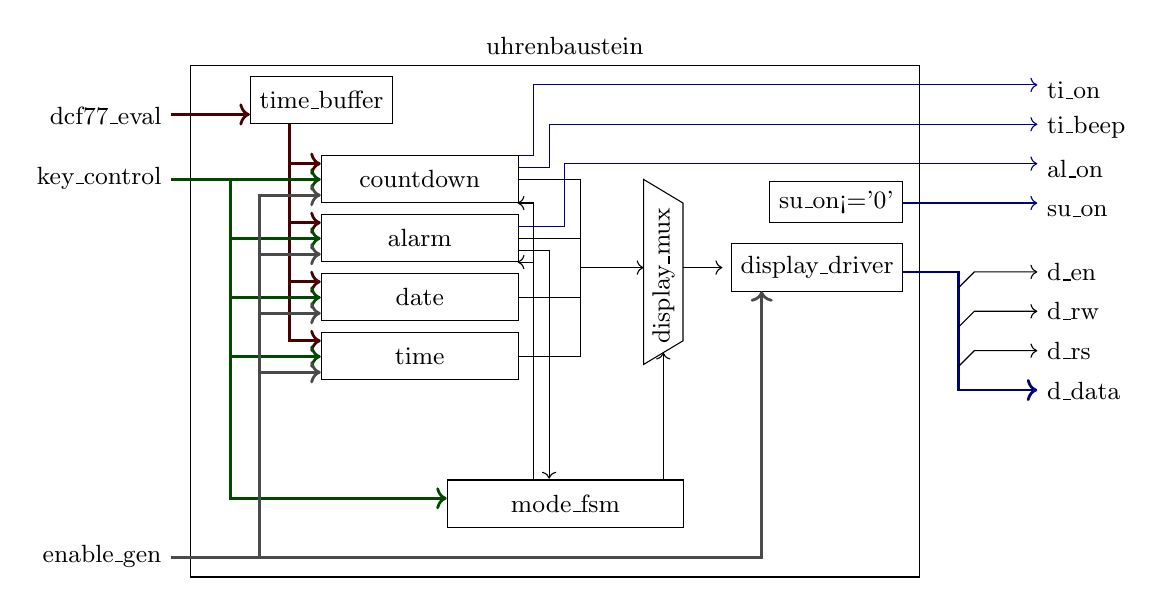
\begin{tikzpicture}[x=1cm,y=1cm,font=\small]
      % top level module
      \node at (4,0.25) {uhrenbaustein};
      \draw[black] (-.75,0) rectangle (8.5, -6.5);

      % individual modules
      \node[rectangle,draw=black,minimum height=0.6cm,minimum width=1.80cm,above right] at (0,-.75) {time\_buffer};
      \node[rectangle,draw=black,minimum height=0.6cm,minimum width=2.5cm,above right] at (.9,-1.75) {countdown};
      \node[rectangle,draw=black,minimum height=0.6cm,minimum width=2.5cm,above right] at (.9,-2.5) {alarm};
      \node[rectangle,draw=black,minimum height=0.6cm,minimum width=2.5cm,above right] at (.9,-3.25) {date};
      \node[rectangle,draw=black,minimum height=0.6cm,minimum width=2.5cm,above right] at (.9,-4) {time};
      \node[rectangle,draw=black,minimum height=0.6cm,minimum width=1.80cm,above left] at (8.3,-2.875) {display\_driver};
      \node[rectangle,draw=black,minimum height=0.6cm,minimum width=3.00cm,above right] at (2.5,-5.875) {mode\_fsm};
       % mux
      \draw (5,-1.45) -- (5.5, -1.75) -- (5.5,-3.5) -- (5,-3.8) -- cycle;
      \node[rotate=90] at (5.25,-2.67) {display\_mux};

      % time signals
      \draw[red!29!black,line width=1pt,->] (-1,-.625) -- (0,-.625);
      \draw[red!29!black,line width=1pt,->] (.5,-1.25) -> (.9,-1.25);
      \draw[red!29!black,line width=1pt,->] (.5,-2) -> (.9,-2);
      \draw[red!29!black,line width=1pt,->] (.5,-2.75) -> (.9,-2.75);
      \draw[red!29!black,line width=1pt,->] (.5,-.75) -- (.5,-3.5) -> (.9,-3.5);
      \node[rectangle,above left] at (-1,-.875) {dcf77\_eval};

      % key status signals
      \draw[green!29!black,line width=1pt,->] (-.25,-1.45)-> (.9,-1.45);
      \draw[green!29!black,line width=1pt,->] (-.25,-2.2) -> (.9,-2.2);
      \draw[green!29!black,line width=1pt,->] (-.25,-2.95) -> (.9,-2.95);
      \draw[green!29!black,line width=1pt,->] (-.25,-3.7) -> (.9,-3.7);
      \draw[green!29!black,line width=1pt,->] (-1,-1.45) -- (-.25,-1.45) -- (-.25,-5.5) -> (2.5,-5.5);
      \node[rectangle,above left] at (-1,-1.7) {key\_control};

      % enable_gen
      \draw[white!29!black,line width=1pt,->] (.125,-6.25) --(.125,-1.65)-> (.9,-1.65);
      \draw[white!29!black,line width=1pt,->] (.125,-2.4) -> (.9,-2.4);
      \draw[white!29!black,line width=1pt,->] (.125,-3.15) -> (.9,-3.15);
      \draw[white!29!black,line width=1pt,->] (.125,-3.9) -> (.9,-3.9);
      \draw[white!29!black,line width=1pt,->] (-1,-6.25) -- (6.5,-6.25) -> (6.5,-2.87);
      \node[rectangle,above left] at (-1,-6.5) {enable\_gen};

      % display data signals
      \draw[->] (3.4,-1.45) -- (4.2, -1.45) --(4.2,-2.57) -> (5,-2.57);
      \draw (3.4,-2.2) -- (4.2, -2.2);
      \draw (3.4,-2.95) -- (4.2, -2.95);
      \draw (3.4,-3.7) -- (4.2, -3.7) -- (4.2,-2.57);

      % status signals modules -> fsm
      \draw[->] (3.4,-2.35) -- (3.8,-2.35) -> (3.8,-5.25);

      % control signals fsm -> modules
      \draw[->] (3.6,-5.25) -- (3.6,-2.5) -> (3.4,-2.5);
      \draw[->] (3.6,-2.5) -- (3.6,-1.75) -> (3.4,-1.75);
      % fsm -> mux
      \draw[->] (5.25,-5.25) -> (5.25,-3.65);
      % mus -> display_driver
      \draw[->] (5.5,-2.57) -> (6,-2.57);

      % Output signals
      \draw[blue!49!black,->](3.4,-1.15) --(3.6,-1.15)--(3.6, -0.25)-> (10, -0.25);
      \node[above right] at (10,-0.55){ti\_on};
      \draw[blue!49!black,->](3.4,-1.3) --(3.8,-1.3)--(3.8, -0.75)-> (10, -0.75);
      \node[above right] at (10, -1.05){ti\_beep};
      \draw[blue!49!black,->](3.4,-2.05) --(4,-2.05)--(4, -1.25)-> (10, -1.25);
      \node[above right] at (10, -1.55){al\_on};
      \node[rectangle,draw=black,above left] at (8.3,-2) {su\_on<='0'};
      \draw[blue!49!black,->] (8.3,-1.75) -> (10,-1.75);
      \node[above right] at (10,-2.05){su\_on};

      % Output display
      \draw[blue!49!black,line width=1pt,->] (8.3,-2.625) -- (9,-2.625) -- (9, -4.125) -> (10, -4.125);
      \draw[->] (9, -2.625) ++(0,-.2) -- ++(.2,.2) -- ++(.8, 0) node[right] {d\_en};
      \draw[->] (9, -3.125) ++(0,-.2) -- ++(.2,.2) -- ++(.8, 0) node[right] {d\_rw};
      \draw[->] (9, -3.625) ++(0,-.2) -- ++(.2,.2) -- ++(.8, 0) node[right] {d\_rs};
      \node[above right] at (10, -4.375){d\_data};

   \end{tikzpicture}
  \end{center}
  \caption{Entity and components of uhrenbaustein}
\end{figure}



In the top level-module Uhrenbaustein the inputs and outputs are supplied to all the submodules.
Besides general information like reset and the clock, this includes characters for the display, the current time and which modul currently reacts to the key input.


\subsection{Implementation}

The module Display Mux receives the display output as a three dimentsional array.
This three dimensional array is generated from the two dimensional outputs of the mudules in uhrenbaustein.
Display Mux then generates a two dimensional array for the display driver.
How the different signals for the display are handed through can be seen in \ref{uhrenbaustein_char}.

The signals from the DCF77 transmitter are only handed to the Time Buffer module. All other modules receive their time signal (\texttt{ctime}) from this module.

The Mode FSM module receives all key inputs as well as the information if the alarm is currently ringing. 
From this information it decides, which module is currently active and reacts to the key input. 
It outputs a vector \texttt{keyboard\_focus[3:0]} that is split into separate signals in Uhrenbaustein, \texttt{'1'} indicating that the module receiving this \texttt{keyboard\_focus} signal is active (\ref{uhrenbaustein_key}).
The module Display mux receives the full vector \texttt{keyboard\_focus[3:0]}, from which it decides which output from the modules is printed on the display.

The output \texttt{su\_on} is set to zero, since the stop watch module is not implemented.

\begin{figure}
  \begin{center}
    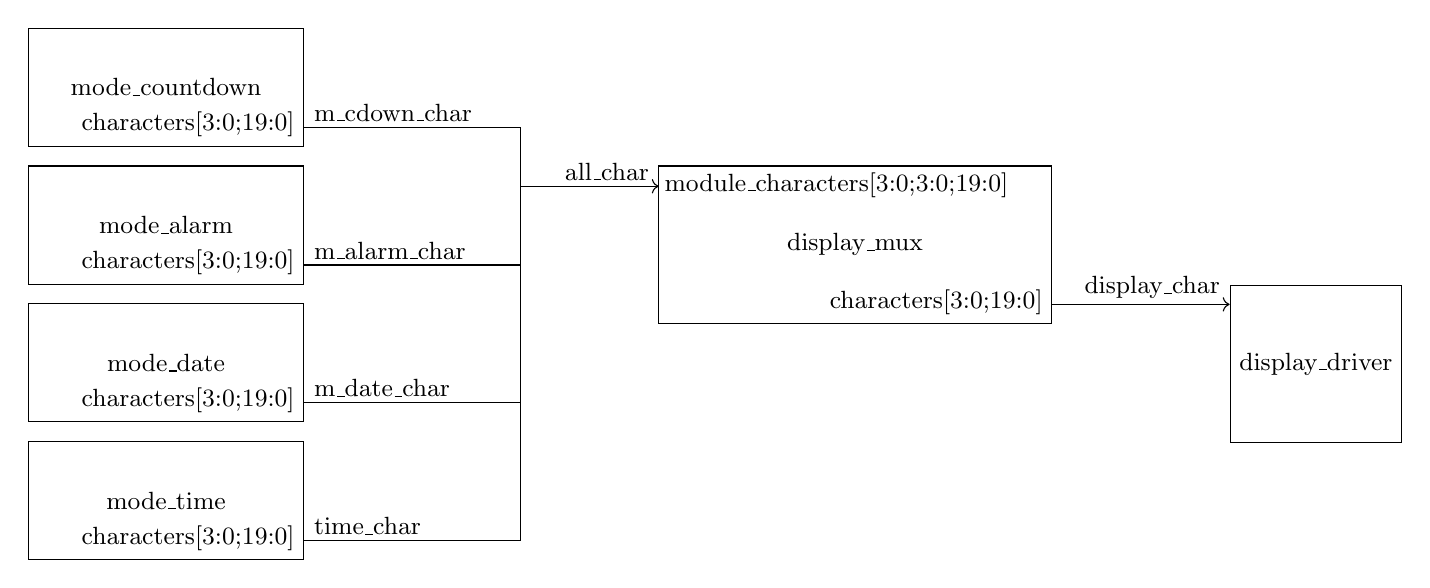
\begin{tikzpicture}[x=1cm,y=1cm,font=\small]

      \label{uhrenbaustein_char}
   %   \draw[help lines] (0, -10) grid (15, 2);

      \node [rectangle, draw=black, minimum height= 1.5cm, minimum width = 3.5cm, above left] at (4, -2) {mode\_countdown};
      \node [above left] at (4, -2) {characters[3:0;19:0]};

      \node [rectangle, draw=black, minimum height= 1.5cm, minimum width = 3.5cm, above left] at (4, -3.75) {mode\_alarm};
      \node [above left] at (4, -3.75) {characters[3:0;19:0]};

      \node [rectangle, draw=black, minimum height= 1.5cm, minimum width = 3.5cm, above left] at (4, -5.5) {mode\_date};
      \node [above left] at (4, -5.5) {characters[3:0;19:0]};

      \node [rectangle, draw=black, minimum height= 1.5cm, minimum width = 3.5cm, above left] at (4, -7.25) {mode\_time};
      \node [above left] at (4, -7.25) {characters[3:0;19:0]};



      \draw[->] (4, -1.75) --(6.75, -1.75) --(6.75, -2.5)->(8.5, -2.5);
      \node [above right] at (4, -1.8) {m\_cdown\_char};
      \draw[-] (4, -3.5) --(6.75, -3.5) --(6.75, -2.5);
      \node [above right] at (4, -3.55) {m\_alarm\_char}; 
      \draw[-] (4, -5.25) --(6.75, -5.25) --(6.75, -2.5);
      \node [above right] at (4, -5.3) {m\_date\_char};
      \draw[-] (4, -7)--(6.75, -7)--(6.75, -2.5);
      \node [above right] at (4, -7.05) {time\_char};
      \node [above left] at (8.5, -2.55) {all\_char};

      \node [rectangle, draw=black, minimum height= 2cm, minimum width = 5cm, above left] at (13.5, -4.25) {display\_mux};
      \node [below right] at (8.45, -2.2) {module\_characters[3:0;3:0;19:0]};
      \node [above left] at (13.5, -4.25) {characters[3:0;19:0]};

      \draw [->] (13.5, -4) -> (15.75, -4);
      \node [above left] at (15.75, -4.05) {display\_char};

      \node [rectangle, draw=black, minimum height=2cm, below right] at (15.75,-3.75) {display\_driver};

    \end{tikzpicture}
  \end{center}
  \caption{Signals for the display}
\end{figure}


\begin{figure}
  \begin{center}
    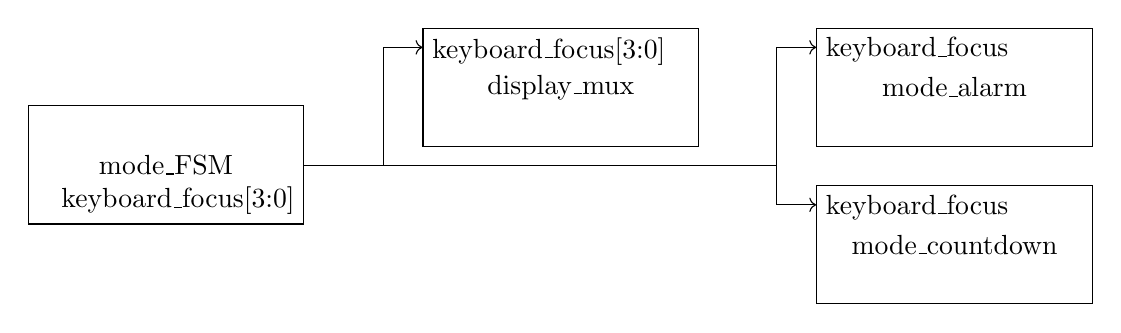
\begin{tikzpicture}
      \label{uhrenbaustein_key}
    %  \draw[help lines] (0, -10) grid (15, 2);

      \node [rectangle, draw=black, minimum height= 1.5cm, minimum width = 3.5cm, above left] at (3, -2.5) {mode\_FSM};
      \node [above left] at (3, -2.5) {keyboard\_focus[3:0]};


      \draw[-] (3, -1.75) --(9,-1.75);
      \draw[->] (9, -1.75) --(9,-0.25)    ->(9.5, -0.25);
      \draw[->] (9, -1.75) --(9,-2.25) ->(9.5,-2.25);
      \draw[->] (4, -1.75) -- (4, -.25) -> (4.5, -.25);

      \node [rectangle, draw=black, minimum height= 1.5cm, minimum width = 3.5cm, below right] at (9.5, 0) {mode\_alarm};
      \node [rectangle, draw=black, minimum height= 1.5cm, minimum width = 3.5cm, below right] at (9.5, -2) {mode\_countdown};
      \node [rectangle, draw=black, minimum height= 1.5cm, minimum width = 3.5cm, below right] at (4.5, 0) {display\_mux};


      \node [below right] at (9.5, 0) {keyboard\_focus};
      \node [below right] at (9.5,-2) {keyboard\_focus};
      \node [below right] at (4.5, 0) {keyboard\_focus[3:0]};

    \end{tikzpicture}
  \end{center}
  \caption{Keyboard Focus signal}
\end{figure}
\subsection{Testing strategy}


\section{Mode Alarm}
  \subsection{Overview}
\begin{figure}
  \begin{center}
    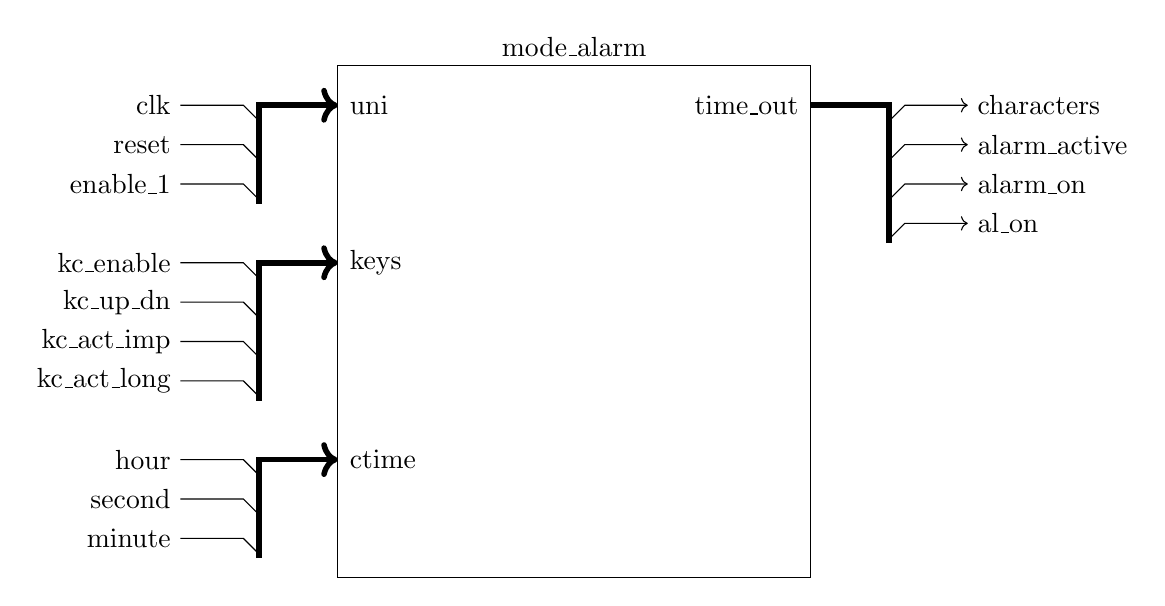
\begin{tikzpicture}
      %\draw[help lines] (-2, -6) grid (4, 2);

      \node[above] at (3,1) {mode\_alarm};

      \draw[line width=2pt,->] (-1, -0.75) |- (0, 0.5) node[right] { uni };

      \draw (-1,  0.5) ++(0,-.2) -- ++(-.2,.2) -- ++(-.8, 0) node[left] {clk};
      \draw (-1,  0)   ++(0,-.2) -- ++(-.2,.2) -- ++(-.8, 0) node[left] {reset};
      \draw (-1,  -.5)   ++(0,-.2) -- ++(-.2,.2) -- ++(-.8, 0) node[left] {enable\_1};



      \draw[line width=2pt,->] (-1, -3.25) |- (0, -1.5) node[right] { keys };

      \draw (-1, -1.5) ++(0,-.2) -- ++(-.2,.2) -- ++(-.8, 0) node[left] {kc\_enable};
      \draw (-1, -2.0) ++(0,-.2) -- ++(-.2,.2) -- ++(-.8, 0) node[left] {kc\_up\_dn};
      \draw (-1, -2.5) ++(0,-.2) -- ++(-.2,.2) -- ++(-.8, 0) node[left] {kc\_act\_imp};
      \draw (-1, -3.0) ++(0,-.2) -- ++(-.2,.2) -- ++(-.8, 0) node[left] {kc\_act\_long};

      \draw[line width=2pt,->] (-1, -5.25) |- (0, -4.0) node[right] { ctime };

      \draw (-1, -4.0) ++(0,-.2) -- ++(-.2,.2) -- ++(-.8, 0) node[left] {hour};
      \draw (-1, -4.5) ++(0,-.2) -- ++(-.2,.2) -- ++(-.8, 0) node[left] {second};
      \draw (-1, -5.0) ++(0,-.2) -- ++(-.2,.2) -- ++(-.8, 0) node[left] {minute};

      \draw[line width=2pt] (7, -1.25) |- (6, .5) node[left] { time\_out };

      \draw[->] (7,  .5) ++(0,-.2) -- ++(.2,.2) -- ++(.8, 0) node[right] {characters};
      \draw[->] (7,   0) ++(0,-.2) -- ++(.2,.2) -- ++(.8, 0) node[right] {alarm\_active};
      \draw[->] (7, -.5) ++(0,-.2) -- ++(.2,.2) -- ++(.8, 0) node[right] {alarm\_on};
      \draw[->] (7,  -1) ++(0,-.2) -- ++(.2,.2) -- ++(.8, 0) node[right] {al\_on};

      \draw (0,1) rectangle (6, -5.5);
    \end{tikzpicture}
  \end{center}
  \caption{Block diagram of mode alarm}
\end{figure}

  \subsection{Implementation}
\begin{figure}
  \begin{center}
    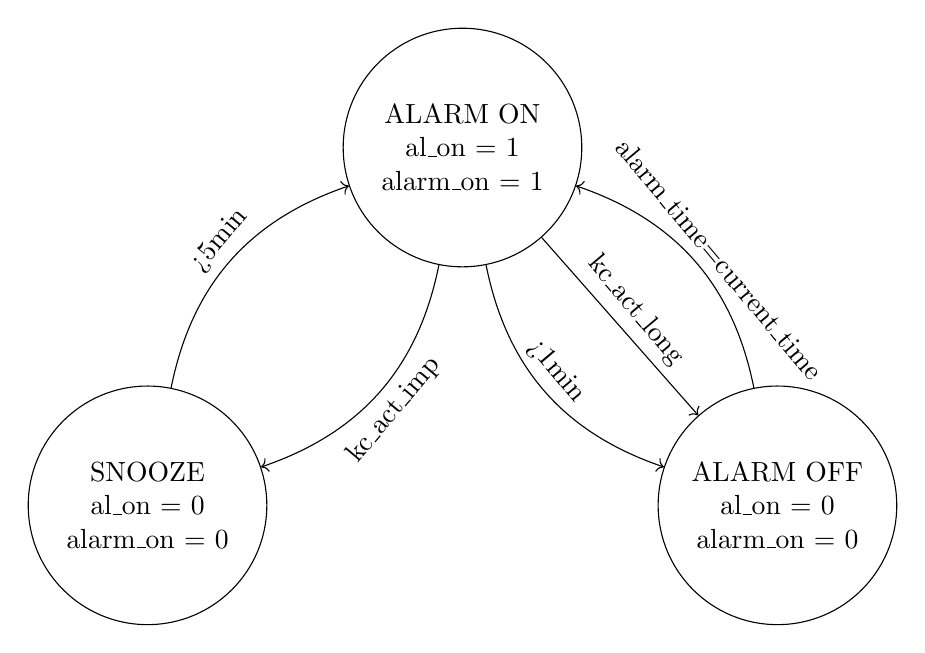
\begin{tikzpicture}[every state/.style={text width=2.5cm,align=center,node distance=.5cm},auto]
      \node[state,                              minimum size=3cm](AlarmOn)  { ALARM ON   \\ al\_on = 1 \\ alarm\_on = 1};               
      \node[state,below=of AlarmOn,xshift=-4cm,yshift=-1cm, minimum size=3cm](Snooze)   { SNOOZE     \\ al\_on = 0 \\ alarm\_on = 0};
      \node[state,below=of AlarmOn,xshift=4cm,yshift=-1cm,minimum size=3cm](AlarmOff) { ALARM OFF  \\ al\_on = 0 \\ alarm\_on = 0 \\ };


      \path[->] (AlarmOn)     edge             node[rotate=-50, shift={(-1,0)}] {kc\_act\_long}               (AlarmOff)
                (AlarmOn)     edge[bend right] node[rotate=-50, shift={(-.7,0)}] { >1min}                     (AlarmOff)
                (AlarmOff)    edge[bend right] node[rotate=-50, shift={(2.25,.5)}] {alarm\_time=current\_time}(AlarmOn)
                (Snooze)      edge[bend left]  node[rotate= 50, shift={(.7,0)}] {>5min}                       (AlarmOn)
                (AlarmOn)     edge[bend left]  node[rotate= 50, shift={(-1,0)}] {kc\_act\_imp}                (Snooze);
 


    \end{tikzpicture}
  \caption{FSM mode alarm}
  \end{center}
\end{figure}

When the alarm is active, mode alarm can be in three states:
  \begin{itemize}
    \item Alarm on
    \item Snooze
    \item Alarm off
  \end{itemize}

   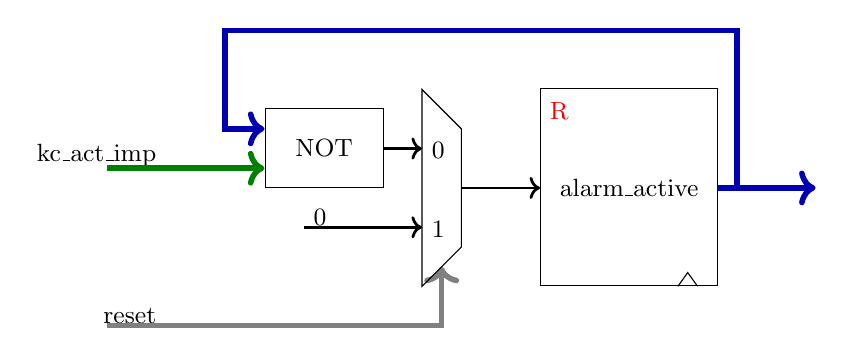
\begin{tikzpicture}[align=center,font=\small,node distance=.5cm,auto]
      %input signals
      \node[above left] at (.25,-1.1){kc\_act\_imp};
      \draw[green!50!black,line width=2pt,->] (-0.5,-1) -- (1.5,-1);
      \node[above right] at (2,-1.85){0};
      \draw[black,line width=1pt,->] (2,-1.75) -> (3.5,-1.75);
      \node[above left] at (.25, -3.1){reset};
      \draw[gray,line width=2pt,->] (-0.5,-3) -- (3.75,-3) -> (3.75,-2.25);

      %internal signals
      \draw[black,line width=1pt,->](3,-.75) -> (3.5,-.75);
      \draw[black,line width=1pt,->](4,-1.25) -> (5,-1.25);

      %+/-
      \node[rectangle,draw=black,minimum height=1cm,minimum width=1.5cm,above right] at (1.5,-1.25) {NOT};
      %mux
      \draw (3.5,0) -- (4,-.5) -- (4,-2) -- (3.5,-2.5)--cycle;
      \node[above right] at (3.5,-1){0};
      \node[above right] at (3.5,-2){1};
      %register
      \node[rectangle,draw=black,minimum height=2.5cm,minimum width=2.25cm,above right] at (5,-2.5) {alarm\_active};
      \node[red,above right] at (5,-.5){R};    
      \draw (6.75,-2.5)--(6.875,-2.325) -- (7,-2.5);

      %output
      \draw[blue!70!black,line width=2pt,->] (7.25,-1.25) -> (8.5,-1.25);
      \draw[blue!70!black,line width=2pt,->] (7.5,-1.25) -- (7.5,.75) -- (1,.75) -- (1,-0.5) -> (1.5,-0.5); 

    \end{tikzpicture}

    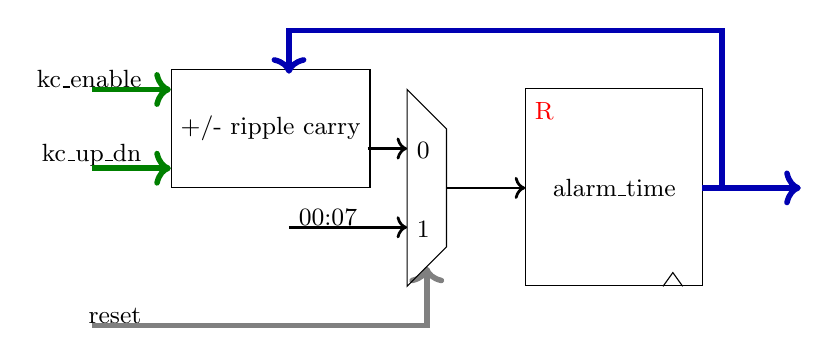
\begin{tikzpicture}[align=center,font=\small,node distance=.5cm,auto]
      %input signals
      \node[above left] at (.25,-.1){kc\_enable};
      \draw[green!50!black,line width=2pt,->] (-0.5,0) -- (0.5,0);
      \node[above left] at (.25,-1.1){kc\_up\_dn};
      \draw[green!50!black,line width=2pt,->] (-0.5,-1) -- (0.5,-1);
      \node[above right] at (2,-1.85){00:07};
      \draw[black,line width=1pt,->] (2,-1.75) -> (3.5,-1.75);
      \node[above left] at (.25, -3.1){reset};
      \draw[gray,line width=2pt,->] (-0.5,-3) -- (3.75,-3) -> (3.75,-2.25);

      %internal signals
      \draw[black,line width=1pt,->](3,-.75) -> (3.5,-.75);
      \draw[black,line width=1pt,->](4,-1.25) -> (5,-1.25);

      %+/-
      \node[rectangle,draw=black,minimum height=1.5cm,minimum width=2.5cm,above right] at (.5,-1.25) {+/- ripple carry};
      %mux
      \draw (3.5,0) -- (4,-.5) -- (4,-2) -- (3.5,-2.5)--cycle;
      \node[above right] at (3.5,-1){0};
      \node[above right] at (3.5,-2){1};
      %register
      \node[rectangle,draw=black,minimum height=2.5cm,minimum width=2.25cm,above right] at (5,-2.5) {alarm\_time};
      \node[red,above right] at (5,-.5){R};
      \draw (6.75,-2.5)--(6.875,-2.325) -- (7,-2.5);

      %output
      \draw[blue!70!black,line width=2pt,->] (7.25,-1.25) -> (8.5,-1.25);
      \draw[blue!70!black,line width=2pt,->] (7.5,-1.25) -- (7.5,.75) -- (2,.75) -> (2,0.2);

    \end{tikzpicture}

   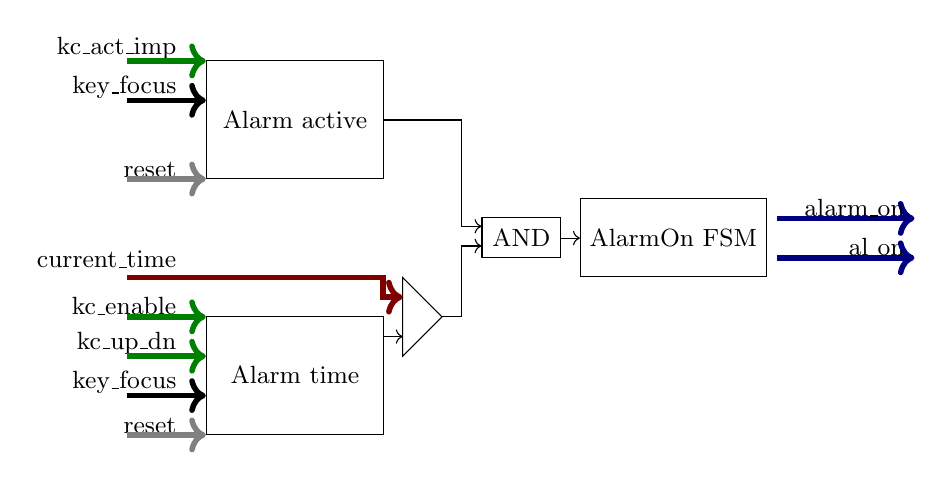
\begin{tikzpicture}[align=center,font=\small,node distance=.5cm,auto]
%       \draw[red] (-3,3) rectangle (9,-4);

    % main modules
      \node[rectangle,draw=black,minimum height=1.5cm,minimum width=2.25cm,above right] at (0.5,1.25) {Alarm active};
      \node[rectangle,draw=black,minimum height=1.5cm,minimum width=2.25cm,above right] at (0.5,-2) {Alarm time};
      \node[rectangle,draw=black,minimum height=1cm,minimum width=2cm,above right] at (5.25,0) {AlarmOn FSM};
      % compare
      \draw (3,0) -- (3.5, -.5) -- (3,-1) -- cycle;
      % AND 
      \node[rectangle,draw=black,minimum height=0.5cm,minimum width=1cm,above right] at (4,0.25) {AND};

      % basic connections
      \draw[->] (2.75,2)  -- (3.75,2) -- (3.75,0.65) -> (4,0.65);
      \draw[->] (2.75,-0.75) -> (3,-0.75);
      \draw[->] (3.5, -0.5) -- (3.75,-0.5) -- (3.75, 0.4) -> (4,0.4);
      \draw[->] (5, 0.5) -> (5.25, 0.5);

      % input
      \node[above left] at (.25,2.65){kc\_act\_imp};
      \draw[green!50!black,line width=2pt,->] (-0.5,2.75) -- (0.5,2.75);
      \node[above left] at (.25,2.15){key\_focus};
      \draw[black,line width=2pt,->] (-0.5,2.25) -- (0.5,2.25);
     %\node[above left] at (.25, 1.65){key\_focus};
     %\draw[red!50!black,line width=2pt,->] (-0.5,1.75) -- (0.5,1.75);
      \node[above left] at (.25, 1.15){reset};
      \draw[gray,line width=2pt,->] (-0.5,1.25) -- (0.5,1.25);


      \node[above left] at (0.25,0){current\_time};
      \draw[red!50!black,line width=2pt,->] (-0.5, 0) -- (2.75,0) -- (2.75,-.25) -> (3,-.25);

      \node[above left] at (.25,-.6){kc\_enable};
      \draw[green!50!black,line width=2pt,->] (-0.5,-.5) -- (0.5,-.5);
      \node[above left] at (.25,-1.1){kc\_up\_dn};
      \draw[green!50!black,line width=2pt,->] (-0.5,-1) -- (0.5,-1);
      \node[above left] at (.25, -1.6){key\_focus};
      \draw[black!50!black,line width=2pt,->] (-0.5,-1.5) -- (0.5,-1.5);
      \node[above left] at (.25, -2.1){reset};
      \draw[gray,line width=2pt,->] (-0.5,-2) -- (0.5,-2);

      % output
      \node[above left] at (9.5,0.15){al\_on};
      \draw[blue!50!black,line width=2pt,->] (7.75,0.75) -> (9.5,0.75);
      \node[above left] at (9.5,0.65){alarm\_on};
      %\draw[blue!30!white,line width=2pt,->] (7.85,0.75) -- (7.85,3.5) -- (1,3.5) -> (1,2.75);
      %\draw[blue!30!white,line width=2pt,->] (8,0.75) -- (8,-2.5) -- (1,-2.5) -> (1,-2);

      \draw[blue!50!black,line width=2pt,->] (7.75,0.25) -> (9.5,0.25);



    \end{tikzpicture}






When the \texttt{ALARM ON} state is entered from the state \texttt{ALARM OFF}, 
the signals \texttt{snooze\_hour} and \texttt{snooze\_minute} are set to the current alarm time. 
These signals are then used to start the alarm again in the \texttt{SNOOZE} state. 
Every time this state is entered, the snooze time is increased by five minutes. 
This is implemented with the same ripple carrier adder that is used to set the alarm time.
Two variables run through it five times, then \texttt{snooze\_hour} and \texttt{snooze\_minute} 
are set to their values. 
This solution was chosen to avoid careless mistakes when implementing the five minute ripple carrier adder.

  \subsection{Testing strategy}


\end{document}
